\documentclass[a4paper,abstract=on,twoside,parskip=full]{scrreprt}
\setlength\parindent{1.5em}

\usepackage[todo]{../../common/naps62}

\hypersetup{pdfauthor={André Martins Pereira}}
\hypersetup{pdftitle={Pre-Thesis: Efficient processing of ATLAS events analysis in platforms with accelerator devices}}

\bibliography{../../common/bib/refs}

% reduce chapter margins
\renewcommand{\chapterheadstartvskip}{\vspace*{-1.6\baselineskip}}

\begin{document}
\pdfbookmark{Cover}{cover}
\pagenumbering{roman}
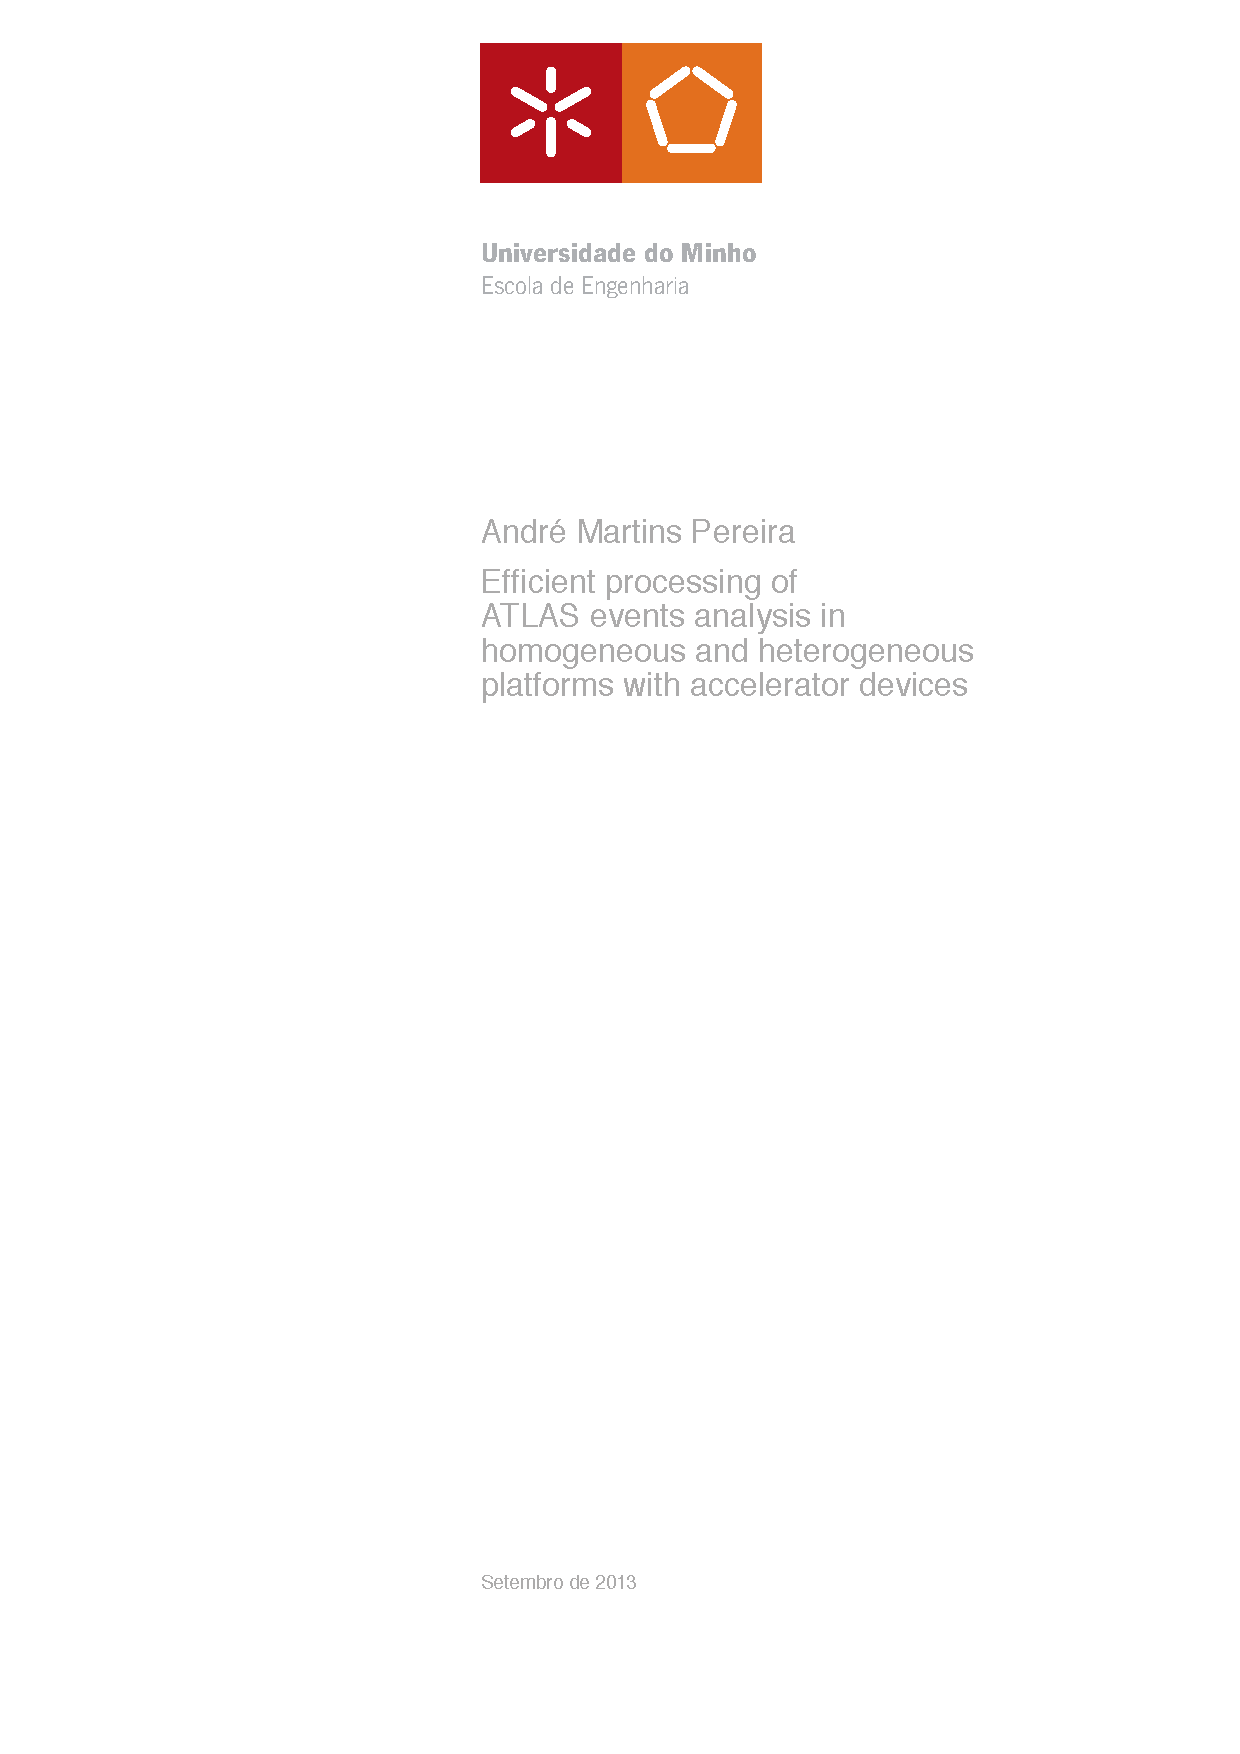
\includepdf[pages=-]{misc/cover-mei}

\pagestyle{fancy}
\renewcommand{\headrulewidth}{0.4pt}
\fancyhead[LO,RE]{}
\fancyhead[LE]{\slshape \leftmark}
\fancyhead[RO]{\slshape \rightmark}
\fancyfoot[RO,LE]{\thepage}%
\fancyfoot[C]{}

\fancypagestyle{plain}{%
  \renewcommand{\headrulewidth}{0.0pt}
  \fancyhead{}
  \fancyfoot[C]{}
  \fancyfoot[RO,LE]{\thepage}
}

\newcommand{\sigspace}[2]{

\begin{minipage}{\columnwidth}%
\vspace{2cm}
\begin{tabular*}{\textwidth}{@{\extracolsep{\fill}}lr}
\hline
{#1} & #2
\end{tabular*}
\end{minipage}%
}


%
% include all tex/ chapter files
%


\pdfbookmark{Resumo}{resumo}
\chapter*{Resumo}

A maior parte das tarefas de análise de dados de eventos no projeto ATLAS requerem grandes capacidades de acesso a dados e processamento, em que q performance de algumas das tarefas são limitadas pela capacidade de I/O e outras pela capacidade de computação.

Esta dissertação irá focar-se principalmente nos problemas limitados computacionalmente nas últimas fases de análise dos dados do detector do ATLAS (as calibrações), complementando uma dissertação paralela que irá lidar com as tarefas limitadas pelo I/O.

O principal objectivo deste trabalho será desenhar, implementar, validar e avaliar uma tarefa de análise mais robusta e melhorada, que envolve aperfeiçoar a performance da reconstrução kinemática de eventos dentro da framework usada para a análise de dados no ATLAS, a ser executada em plataformas de computação heterogénea baseada em CPUs multicore acoplados com placas PCI-E com dispositivos many-core, tais como o \intel Xeon Phi e/ou os dispositivos GPU \nvidia Fermi/Kepler.

Uma aplicação de análise será usada como caso de estudo, desenvolvida pelo grupo LIP, para melhorar a reconstrução kinemática, bem como restruturar e paralelizar outras regiões críticas desta análise.

Uma framework experimental, GAMA, será usada para automatizar (i) a distribuição de carga pelos recursos disponíveis e (ii) a gestão transparente de dados através do ambiente de memória física distribuída, entre a memória partilhada do CPU multicore e da memória dos dispositivos many-core. Ela será comparada com outra framework similar, OpenACC, em termos de performance, tempo de desenvolvimento e usabilidade.

\newpage \pdfbookmark{Abstract}{abstract}
\chapter*{Abstract}

Most event data analysis tasks in the ATLAS project require both intensive data access and processing, where some tasks are typically I/O bound while others are compute bound.

This dissertation work will mainly focus on compute bound issues at the latest stages of the ATLAS detector data analysis (the calibrations), complementing a parallel dissertation work that addresses the I/O bound issues.

The main goal of the work is to design, implement, validate and evaluate an improved and more robust data analysis task which involves tuning the performance of the kinematical reconstruction of events within the framework used for data analysis in ATLAS, to run on computing heterogeneous platforms based on multi-core CPU devices coupled to PCI-E boards with many-core devices, such as the \intel Xeon Phi and/or the \nvidia Fermi/Kepler GPU devices.

As a case study, an analysis application will be used, developed by the LIP research group, to tune the kinematical reconstruction, as well as restructure and parallelize other critical areas of this analysis.

An experimental framework, GAMA, will be used to automate (i) the workload distribution among the available resources and (ii) the transparent data management across the physical distributed memory environment between the shared multi-core memory and the many-core device memory. It will be compared against a similar concurrent framework, OpenACC, in terms of performance, development time and usability.

\newpage
\pagenumbering{arabic}


\pdfbookmark{Contents}{contents}
\tableofcontents

\newpage \pdfbookmark{Glossary}{glossary}
\chapter*{Glossary}
\begin{acronym}
  \acro{Event}{Head-on collision between two particles at the LHC}
  \acro{Combination}{A set of two leptons and two jets}
  \acro{LHC}{Large Hardron Collider particle accelerator}
  \acro{ATLAS project}{Experiment being conducted at the LHC with an associated particle detector}
  \acro{LIP}{Laboratório de Instrumentação e Física Experimental de Partículas, Portuguese research group working in the ATLAS project}
  \acro{CERN}{European Organization for Nuclear Research, which results from a collaboration from many countries to test HEP theories}
  \acro{HEP}{High Energy Physics}
  \acro{Analysis}{Application developed to process the data gathered by the ATLAS detector and test a specific HEP theory}
  \acro{Accelerator device}{Specialized processing unit connected to the system by a PCI-Express interface}
  \acro{CPU}{Central Processing Unit, which may contain one or more cores (multicore)}
  \acro{GPU}{Graphics Processing Unit}
  \acro{GPGPU}{General Purpose Graphics Processing Unit, recent designation to  scientific computing oriented GPUs}
  \acro{DSP}{Digital Signal Processor}
  \acro{MIC}{Many Integrated Core, accelerator device architecture developed by \intel, also known as Xeon Phi}
  \acro{QPI}{Quickpath Interconnect, point-to-point interconnection developed by \intel}
  \acro{HT}{HyperTransport, point-to-point interconnection developed by the HyperTransport Consortium}
  \acro{NUMA}{Non-Uniform Memory Access, memory design where the access time depends on the location of the memory relative to a processor}
  \acro{ISE}{Instruction Set Extensions, extensions to the CPU instruction set, usually SIMD}
  \acro{Homogeneous system}{Classic computer system, which contain one or more similar multicore CPUs}
  \acro{Heterogeneous system}{Computer system, which contains a multicore CPU and one or more accelerator devices}
  \acro{SIMD}{Single Instruction Multiple Data, describes a parallel processing architecture where a single instruction is applied to a large set of data simultaneously}
  \acro{SIMT}{Single Instruction Multiple Threads, describes the processing architecture that \nvidia uses, very similar to SIMD, where a thread is responsable for a subset of the data to process}
  \acro{SM/SMX}{Streaming Multiprocessor, SIMT/SIMD processing unit available in \nvidia GPUs}
  \acro{Kernel}{Parallel portion of an application code designed to run on a CUDA capable GPU}
  \acro{Host}{CPU in a heterogeneous system, using the CUDA designation}
  \acro{CUDA}{Compute Unified Device Architecture, a parallel computing platform for GPUs}
  \acro{OpenMP}{Open Multi-Processing, an API for shared memory multiprocessing}
  \acro{OpenACC}{Open Accelerator, an API to offload code from a host CPU to an attached accelerator}
  \acro{GAMA}{GPU and Multicore Aware, an API for shared memory multiprocessing in platforms with a host CPU and an attached CUDA enabled accelerators}
  \acro{Speedup}{Ratio of the performance increase between two versions of the code. Usually comparing single vs multithreaded applications.}

  bottleneck
\end{acronym}

\newpage \pdfbookmark{List of Figures}{figures}
\listoffigures
\newpage


\pagenumbering{arabic}

\chapter{Introduction}
\label{Introduction}

\begin{quote}
\textit{The dissertation is first presented by contextualizing the scientific background of CERN and LIP organizations, as well as their current research projects, which are closely involved in this work. The motivation for the dissertation is presented in section \ref{Motivation}, with the problem contextualized from a physics perspective in subsection \ref{TopQuarkSystem}. The Goals, subsection \ref{Goals}, states the objectives to be achieved by this work, in terms of improving the research and application development quality by implementing a set of solutions for homogeneous and heterogeneous systems, while assessing the efficiency and usability of hardware accelerators in the latter. The scientific contribution of this work is presented in subsection \ref{ScientificContribution}. Subsection \ref{DissertationStructure} overviews the structure of this dissertation.}
\end{quote}

\section{Context}
\label{Context}

The European Organization for Nuclear Research \cite{CERN} (CERN, acronym for \textit{Conseil Européen pour la Recherche Nucléaire}) is a consorcium of 20 european member countries with the purpose of operating the largest particle physics laboratory in the world. Founded in 1954, CERN is located in the border between France and Switzerland, and employs thousands of scientists and engineers representing 608 universities and research groups and 113 different nationalities.

CERN research focus on the basic constituents of matter, which started by studying the atomic nucleus but quickly moved into high energy physiscs (HEP), focusing on the interaction between particles. The instrumentation used in the nuclear research, physics-wise, is essentially divided into particle accelerators and detectors, alongside with the facilities necessary for delivering the protons to the accelerators. The purpose of the accelerator is to speed up groups of particles close to the speed of light, in opposite directions, and collide them in the detectors (this collision is called an event). The detectors record various characteristics, such as energy and momentum, of particles resultant from complex decay processes of the original particles. These experiments are performed to test and validate specific HEP theories by comparing the results of the collision to the expected theoretical model.

It started with a small low energy particle accelerator, the Proton Synchrotron \cite{CERN:PS} inaugurated in 1959, but the facilities were iteratively being upgraded and expanded. The current facilities are constituted by the older accelerators (some decomissioned while others are still functional) and detectors, as well as the newer Large Hadron Collider (LHC) \cite{CERN:LHC} high energy particle accelerator which is located 100 meter underground and has a 27 km circuference length. There are currently seven experiments running on the LHC: CMS \cite{CERN:CMS}, ATLAS \cite{CERN:ATLAS}, LHCb \cite{CERN:LHCb}, MoEDAL \cite{CERN:MoEDAL}, TOTEM \cite{CERN:TOTEM}, LHC-forward \cite{CERN:LHCf} and ALICE \cite{CERN:ALICE}. Each of these experiments has their own detector on the LHC and conduct similar or different experiments, but with the use of distinct technologies and research approaches. Currently one of the most popular researches being conducted is the validation of the Higgs boson theory. During the next year the LHC will be upgraded to increase its luminosity (amount of energy of the particle beams that it accelerates).
\todo{Fonte disto do upgrade}

Approximately 600 millions of collisions occur every second in each of the experiment's detectors at the LHC, where the detectors react to the particle interaction and produce electric signals, generating massive amounts of raw data. It's estimated that all the detectors combined produce 25 petabytes of data per year \cite{CERN:DATA1,CERN:DATA2}. CERN does not have the financial resources to have the computational power to process all the data, which motivated the creation of the Worldwide LHC Computing Grid \cite{CERN:WLHCCG}, a distributed computing infrastructure that uses the resources of scientific community for data processing. The grid is organized in a hierarchy divided in 4 tiers. Each tier is made by one or more computing centers and has a set of specific tasks and services to perform, such as store, filter, refine and analyse all the data gathered at the LHC.

The Tier-0 is the data center located at CERN. It provides 20\% of the total grid computing capacity, and its objective is to store and reconstruct the raw data gathered at the detectors in the LHC into meaningful information, usable by the remaining tiers. The data is received on a format designed for this reconstruction, with information about detector and software diagnostics. After the reconstruction the data has a different formats, the Event Summary Data (ESD) and Analysis Object Data (AOD), each one with different purposes, containing information of the reconstructed objects and calibration parameters, and can be used for early analysis. This tier distributes the raw data and the reconstructed output by the 11 Tier-1 computational centers, spread among the different countries that are members of CERN.

Tier-1 computational centers are responsible for storing a portion of the raw and reconstructed data and provide support to the grid 24/7. In this tier, the reconstructed data suffers more reprocessing, in order to refine it by filtering only relevante information and reducing the size of the data, now in Derived Physics Data (DPD) format, that is then transferred to the Tier-2 computational centers. The size of the data for an event is reduced from ~3 MB (raw) to ~10 kB (DPD). This tier also stores the outputs of the simulations performed at Tier-2. The Tier-0 center is connected to the 11 Tier-1 centers by high bandwidth optical fiber links, which consists of the LHC Optical Private Network.

There are around 140 Tier-2 computational centers around the world. Their main purpose is to perform Monte-Carlo simulations with the data received from the Tier-1 centers, but also perform a portion of the events reconstructions. The Tier-3 centers range from university clusters to small personnal computers, and they perform most of the events reconstruction and final data analysis. In the CERN related groups terminology, an analysis is a denomination for an application which is designed to process a given amount of data in order to test a specific HEP theory by providing physically relevant information about events that may support the said theory.

\section{LIP Research Group}
\label{LIP}

The Laboratório de Instrumentação e Física Experimental de Partículas (LIP) \cite{LIP} is a portuguese scientific and technical association for research on experimental high energy physics and associated instrumentation. LIP has a strong collaboration with CERN as it was the first scientific organization Portugal has joined, in 1986. It has laboratories in Lisbon, Coimbra and Minho and 170 people employed. LIP researchers have produced several applications for testing various HEP theories of the ATLAS experiment that use Tier-3 computational resources for data analysis. Most of the analysis applications use home-grown frameworks, such as the LipCbrAnalysis and LipMiniAnalysis.

This dissertation work results from a close cooperation between the Department of Informatics of the University of Minho and the LIP laboratory in Minho.

\todo{Falar aqui do que se trata o trabalho ou referir que está explicado mais a frente?}

\section{Motivation, Goals \& Scientific Contribution}
\label{Motivation}

With an increase of events and, consequently, the data being produced by the detectors at the LHC, specifically in the ATLAS experiment, the research groups will need a bigger budget for aquiring and maintaining computational resources due to an increase of analysis to perform. To add up to this data increase, research groups working on the same experiment have a positive rivalry to be the first find and publish relevant results. The finding of these results is directly related to the amount of events processed, meaning that groups with more computational resources are one step ahead.

Better results are not only obtained by increasing the amount of events analyzed; it is important to take into account the quality of each analysis. The ATLAS detector has an experimental resolution of 2\%, meaning that each measured value for a characteristic of a resultant particle of a collision might not be real and, therefore, the analysis will have an error associated. It is possible to improve the analysis quality but it will increase its execution time, creating a trade-off between events to analyze and their quality. This issue will be presented in the context of this dissertation with more detail on subsection \ref{TopQuarkSystem}.

One of the most important analysis being conducted by LIP is related to the Top Quark physics and the Higgs Boson. An application was devised that reconstructs an event following the theoretical model of Top Quark decay and then also attempts to reconstruct the associated Higgs Boson. Each event can be reconstructed several times, with some of its parameters slightly varied by a random offset (with a maximum magnitude of 2\% of the original value), and by chosing the reconstruction that satisfies the most the theoretical model a better solution is obtained, overcoming the experimental resolution of the ATLAS detector. The more reconstructions per event are performed the longer will take to process an event. The theoretical model for this system is presented in subsection \ref{TopQuarkSystem} and the analysis application in chapter \ref{Application}.

While investing in the upgrade of the computational resources of the research group is a valid option to deal with the increase of events to analyze, it is also necessary to take into account if the current resources are being efficiently used by the analysis applications. Also, hardware is not necessarily getting faster, but wider by increasing the number of cores per chip (see chapter \ref{TechnologicalBackground}), which can cause big investments to result in small improvements. Current computing clusters are constituted of systems with one or more multicore CPUs (homogeneous systems) and some even utilizing hardware accelerators, very efficient for specific problem domains (heterogeneous systems). It is important to have a knowledge of these newer architectures in order to develop efficient applications that resort to parallelism in order to better use all the resources available in a system. Programming for such architectures (multicore CPUs and hardware accelerators) requires a set of skills and experience that most physicists (usually self-taught programmers) do not have, causing poorly optimized applications to be developed.

Increasing the efficiency of an application by resorting to parallelism enables the possibility of performing more reconstructions per event and more events to be processed, while using all the potential of the available computational resources and avoiding needless investments in hardware upgrades.

\subsection{The Top Quark system and Higgs boson decay}
\label{TopQuarkSystem}

In the LHC two proton beams are accelerated close to the speed of light in opposite directions, set to collide inside a specific particle detector. From this head-on collision results a chain reaction of decaying particles, from which only some of the final particles react with the detector for recording their characteristics. One of the experiments being conducted at the ATLAS detector is related to the discovery of new Top Quark physics. The schematic representation of the Top Quark decay (the \ttbar system), resulting from a head-on collision of two protons, is presented in figure \ref{fig:TopQuarkDecay}.

\begin{figure}[!htp]
	\begin{center}
		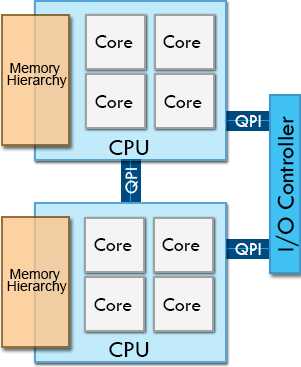
\includegraphics[scale=0.5]{../../common/img/numa_qpi.png}
		\caption{Schematic representation of the \ttbar system.}
		\label{fig:TopQuarkDecay}
	\end{center}
\end{figure}

The ATLAS detector is able to record the characteristics of Bottom Quarks, which are detected as a jet rather than a single particle, and leptons, the muon (that has a positive charge) and electron (with a negative charge). However, the neutrinos do not react with the detector and, therefore, their characteristics are not recorded. To reconstruct the Top Quarks, necessary for researching their properties, it is necessary to have the information of all the final particles, so the neutrino characteristics must be determined. This is possible to do as the \ttbar system obeys a set of properties, and using the information of the quarks and leptons the neutrinos characteristics are analitically calculated. The process of reconstructing the neutrinos is referred as kinematical reconstruction. The reconstruction of the whole \ttbar system has a degree of certainty associated, which determines its quality. The quality of these reconstructions directly affects the quality of the research being conducted by LIP.

The amount of Bottom Quark jets and leptons detected may vary between events, due to other reactions occurring at the same time of the Top Quark decay. As represented in figure \ref{fig:TopQuarkDecay}, it is needed 2 jets and 2 leptons to reconstruct the \ttbar system, but the data for an event may have many of these particles associated. To obtain the best reconstruction for the \ttbar system of a given event it is necessary to reconstruct the respective neutrinos and then the whole system for every combination of 2 jets and 2 leptons, and only chose the most accurate reconstruction.

Another factor affecting the quality of the reconstruction is the experimental resolution of the ATLAS particle detector, which associates an error of 2\% with every measurement made. If the measurements of the jets and leptons are not precise enough the kinematical reconstruction will produce inaccurate neutrinos and affect the overall reconstruction of an event, which might render an event with relevant physics useless. It is possible to overcome this problem by performing the kinematical reconstruction, and then the whole \ttbar system reconstruction, a large amount of times for each combination of 2 Bottom Quark jets with 2 leptons, with a random variation to the particle characteristics (momentum, energy and mass) of a maximum magnitude of 2\% of the original value. The amount of variations performed per combination will directly impact the final quality of the event reconstruction, as more of the search space (defined by the experimental resolution error) is covered compared to performing a single reconstruction. The more variations are performed the more likely it is to find the best possible reconstruction of the \ttbar system.

The look for the Higgs Boson is also part of the research being conducted at LIP. Figure \ref{fig:HiggsBosonDecay} schematizes the Higgs Boson and Top Quark decay. It is possible to reconstruct the Higgs Boson from the two Bottom Quark jets that it decays to, and it can be performed alongside the \ttbar system reconstruction. This adds at least two more jets to the event information, and it is not possible to know before the reconstruction which jets belong to the Higgs decay or the Top Quark decay. Considering this, the Higgs reconstruction must be performed after the \ttbar system reconstruction, in such a way that the jets chosen to reconstruct it must not be the ones used in the \ttbar system reconstruction. Adding this new jets increases the number of jets/leptons combinations to test in the kinematical reconstruction, and for each \ttbar system reconstruction the Higgs must be also reconstructed. Now, the quality of the event reconstruction depends on the quality of both \ttbar system and Higgs Boson reconstructions.

\begin{figure}[!htp]
	\begin{center}
		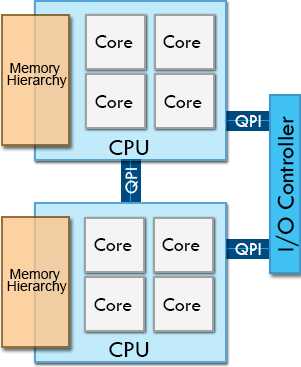
\includegraphics[scale=0.5]{../../common/img/numa_qpi.png}
		\caption{Schematic representation of the \ttbar system with the Higgs Boson decay.}
		\label{fig:HiggsBosonDecay}
	\end{center}
\end{figure}

This specific analysis of events presented is performed by an application developed by LIP researchers, the \tth. The application receives input data file with a set of events and reconstructs the \ttbar system and the Higgs Boson for each event using the processes described. These files are usually 1 GB long and the LIP research requires that hundreds of them are processed by the same application, considering a specific experiment such as the presented in this subsection. A in-depth computational analysis of \tth is presented in chapter \ref{Application}, where its flow is presented, it is characterized in terms of various metrics (such as computational intensity) and the critical regions are identified.

\subsection{Goals}
\label{Goals}

By increasing the performance of the Top Quark and Higgs Boson reconstructions it is possible to perform more variations per event, increasing the quality of the results, and increase the throughput of events processed. The objective of this dissertation work is to take a sequential application made by physicists, which the main concern during its development was the correcteness of the code rather than its performance, the \tth, and improve its efficiency by (i) identifying the bottlenecks and optimizing the code, (ii) increasing the performance by resorting to parallelism for homogeneous and heterogeneous systems, assessing the efficiency (performance and usability) of hardware accelerators for this type of problem, and (iii) the development of a simple scheduler for managing the workload among various instances of the same sequential or parallel application (i.e. an application which needs to process a large set of separate input files) on homogeneous systems.

This work will give a inside perspective of how scientific applications are being developed by programmers with little to no background in computer science, and possibly define a set guidelines for coding of efficient applications and the usage of parallelism in such applications. All the changes that will be made to the \tth application, including the introduction of parallelism, will be as independent as possible from the context of this specific problem, in such a way that they might be portable to other applications without requiring major modifications. The work will be structured, implementation wise, so that the parallelization mechanisms and the scheduler are possible to be improved and transformed in a tool used by the researchers at LIP.

\subsection{Scientific Contribution}
\label{ScientificContribution}

This dissertation work aims to improve the quality of a specific research field conducted by LIP, provide a set of tools and know-how to improve the performance of similar scientific applications and expose the problematic of unefficient usage of computational resources. By improving the quality of the research, LIP will gain an advantage over other research groups in the look for new Top Quark physics and in the Higgs Boson discovery. By experiencing the process of optimizating scientific applications of this kind it is possible to provide physicists with some know-how and tools for optimization and parallelization with the goal of increasing the performance in future applications. By developing applications that efficiently use all the computational resources available it is possible to reduce the investment in new hardware, which otherwise would have small pratical returns.

\section{Dissertation Structure}
\label{DissertationStructure}

This dissertation has 5 chapters and their summary is presented below:

\begin{description}
	\item[Introduction] \hfill \\
	The dissertation is first presented by contextualizing the scientific background of CERN and LIP organizations, as well as their current research projects, which are closely involved in this work. The motivation for the dissertation is presented in section \ref{Motivation}, with the problem contextualized from a physics perspective in subsection \ref{TopQuarkSystem}. The Goals, subsection \ref{Goals}, states the objectives to be achieved by this work, in terms of improving the research and application development quality by implementing a set of solutions for homogeneous and heterogeneous systems, while assessing the efficiency and usability of hardware accelerators in the latter. The scientific contribution of this work is presented in subsection \ref{ScientificContribution}. Subsection \ref{DissertationStructure} overviews the structure of this dissertation.
	\item[Technological Background] \hfill \\
	This chapter presents the current technological state of the art in terms hardware and software. Hardware-wise, both homogeneous and heterogeneous system architectures and details are presented in sections \ref{HomogeneousSystems} and \ref{HeterogeneousSystems}, respectively. A contextualization of current hardware accelerators is also made in the latter. Software-wise is presented in section \ref{Software}. Various frameworks and libraries are presented for homogeneous systems and accelerators in sections \ref{pThreads}, \ref{OpenMP}, \ref{MPI} and \ref{CUDA}. Section \ref{HeterogeneousFrameworks} presents the available frameworks for parallelization in heterogeneous systems. Finally, current solutions for profiling and debugging parallel applications is presented in section \ref{ProfilingDebugging}.
	\item[\tth Application] \hfill \\
	The \tth application for event reconstruction is presented in this chapter. Its dependencies are presented. The flow of the application is presented in section \ref{Application:Flow}, accompanied by a schematic representation. Its main functions are presented and the schematic flow is compared against a callgraph of the application to help understanding what happens in each of the most important functions. The critical region is identified in section \ref{CriticalRegion} and characterized in subsection \ref{ComputationalCharactrization}. Some initial optimizations to the code are presented in subsection \ref{InitialOptimizations}.
	\item[Parallelization Approaches] \hfill \\
	For different parallelization alternatives are presented in this chapter. For homogeneous systems, a shared memory parallelization is discussed in section \ref{Parallelization:SharedMem}, where the abstract heuristic used is shown, and the implementation and a performance analysis are presented in subsections \ref{SharedMemImplementation} and \ref{SharedMemPerformance}, respectively. For heterogeneous systems using hardware accelerators, two alternatives are presented: using GPU as an accelerator, in section \ref{Parallelization:GPU}, with its implementation and performance discussed and analyzed in subsections \ref{GPUImplementation} and \ref{GPUPerformance}; using the \intel Xeon Phi as an accelerator in section \ref{Parallelization:MIC} and its implementation discussed in subsection \ref{MICImplementation}. A software scheduler for managing workload distribution among applications for homogeneous shared memory systems is presented in section \ref{Parallelization:Scheduler}. Its implementation details and performance analysis are shown in subsections \ref{SchedulerImplementation} and \ref{SchedulerPerformance}.
	\item[Conclusions \& Future Work] \hfill \\
	This chapter concludes the dissertation, presenting an overview of the results obtained by the work developed, on both homogeneous and heterogeneous systems. Guidelines for future work, on improving the test case application and providing parallel solutions abstracted from the programmer for future application development, are presented.
\end{description}

\chapter{Technological Background}
\label{TechnologicalBackground}

\section{Hardware}
\label{Hardware}

Computer systems started with a very simple design, where a processing chip (CPU) is connected to a data storage unit (memory). The complexity of the processing chips increased, as well as the memory, specifically with the use of an hierarchy model, and current systems are usually made from multicore CPUs and various types of memory.

The most common are homogeneous systems, constituted from one or more CPU chips with their own memory bank (RAM memory) and interconnected by a specific interface, which is manufacturer-specific. Although the system uses a shared memory model, where all the data is always available for each CPU, in the case of a multiple CPU system, since the memory is distributed in one bank per CPU the system will have a Non Unified Memory Access (NUMA) pattern. This means that the access time of a CPU to a piece of memory in its memory bank will be faster than accessing memory on the other CPU bank. It is important to have the data on the CPU memory bank that the application will run to avoid the increased costs of NUMA.

With the emerging use of hardware designed for specific computing domains, hardware accelerators, which purpose is to efficiently solve a small range of problems, as opposed to general purpose CPU chips. This marked the begining of heterogeneous systems, where one or more CPU chips, operating in a shared memory environment, are accompanied by one or more hardware accelerators. The CPUs and accelerators operate in a distributed memory model, meaning that data must be explicitly passed from the CPU to the accelerator and vice-versa.

\begin{figure}[!htp]
	\begin{center}
		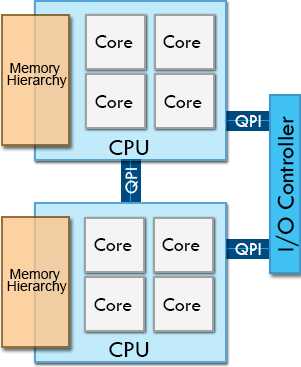
\includegraphics[scale=0.5]{../../common/img/numa_qpi.png}
		\caption{Schematic representation of a heterogeneous system.}
		\label{fig:HeterogeneousSystem}
	\end{center}
\end{figure}

Figure \ref{fig:HeterogeneousSystem} presents a schematic representation of a heterogeneous system. Note the interconnection between CPUs, responsible for the NUMA pattern, and that both CPUs must use the same interface to communicate with the hardware accelerators. This interface has a high latency for memory transfers, making it a critical spot in applications performance.

\subsection*{CPU chips}
\label{CPUChips}

Gordon Moore predicted in 1965 that for the following ten years the number of transistors on CPU chips would double every 1.5 years \cite{MooreLaw}. This was later known as the Moore's Law and it is expected to remain valid at least up to 2015. This enabled the increase in CPU chips clock frequency by the same factor as the transistors. Software developers did not expend much effort optimizing their applications and only relied on the hardware improvements to make them faster.

Due to thermal dissipation issues, the clock frequencies of CPU chips started to stall in 2005. Manufacturers shifted from making CPUs faster to increasing their throughput by adding more cores to a single chip, reducing their energy consumption and operating temperature. This marked the beggining of the multicore and parallel computing era, where every new generation of CPUs get wider, while their clock frequencies remain steady.

The CPU chips are designed as general purpose computing devices, based on a simple design consisting of small processing units with a very fast hierarchized memory attached (cache, which purpose is to reduce the slow accesses to global memory), and all the necessary data load/store and control units. They are capable of delivering a good performance in a wide range of operations, from executing simple integer arithmetic to complex branching and SIMD (single instruction multiple data, explained below) instructions. A single CPU core implements various mechanisms for improving the performance of applications, at the instruction level, with the most important explained next:

\begin{description}
	\item[\textit{ILP}] instruction level parallelism (ILP) is the overlapping of instructions, performed at the hardware or software level, which otherwise would run sequentially. At the software level it is denominated as static parallelism, where compilers try to identify which instructions are independent, i.e., the result of one does not affect the outcome of the other, and can be executed at the same time, if the hardware has resources to do so. At the hardware level, ILP can be referred as dynamic parallelism as the hardware dynamically identifies which instructions execution can be overlapped while the application is running. The three mechanisms presented next allow for ILP to be used.
	\begin{description}
		\item[\textit{Out of order execution}] is the execution of instructions in different order as they are organized in the application binary, without violating any data dependencies. This technic exposes ILP, which otherwise would not be possible.
		\item[\textit{Super Scalarity}] is a mechanism which allows dispatching a certain amount of instructions to the respective arithmetic units in each clock cycle, increasing the throughput of the CPU. Instructions that are not data dependent can run simultaneously, as long as they use different arithmetic units.
		\item[\textit{Pipelining}] is the division of an instruction execution in stages. This stages range from loading the data, instruction execution in, also pipelined, arithmetic units and writing the results back to memory. This allow, as an example, for an instruction to be loaded while other is being executed. Moreover, inside an arithmetic unit, multiple instructions can be simultaneously executed, as long as they are in different stages.
	\end{description}
	\item[\textit{Speculative execution}] is the usage of branch prediction (predict which branch of a conditional jump will be executed, before knowing the condition result), which can use complex algorithms based on previous conditional jumps, and start executing instructions in the predicted branch. If the prediction fails, the results are trashed and the other branch is executed. Current hardware is capable of executing both branches of a conditional jump and accept the one correct once the condition is resolved.
	\item[\textit{Vector instructions}] are a special set of intructions based on the SIMD model, where a single instruction is applied to a large set of data simultaneously. CPU instruction sets offer special registers and instructions that allow to take a chunk of data and execute an instruction to modify it in a special arithmetic usage. One of the most common examples is addition of two vectors. The hardware is capable of adding a given number of elements of the vectors simultaneously. This optimization is done at compile time.
	\item[\textit{Multithreading}] is the execution of multiple threads in the same core. This is possible by replicating part of the CPU resources, such as registers, and can lead to a more efficient utilization of the core hardware. If one of the threads is waiting for data to execute the next instruction, other thread can resume execution while the first is stalled. It also can allow a better usage of resources which would otherwise be idle during the execution of a single thread. If multiple threads are working on the same data, multithreading can reduce the synchronization between them and lead to a better cache usage.
\end{description}

A schematic representation of a modern CPU chip is presented in figure \ref{fig:CPUChip}. It is constituted of several, possibly multithreaded, cores, each with its own level 1 and 2 caches and a level 3 cache shared among all cores. This level 3 cache allows fast comunication and synchronization of data between cores of the same CPU.

\begin{figure}[!htp]
	\begin{center}
		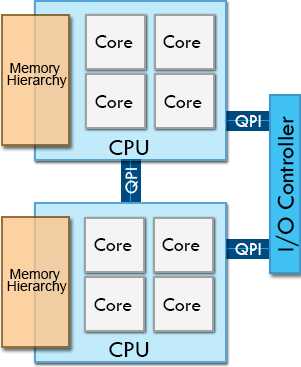
\includegraphics[scale=0.5]{../../common/img/numa_qpi.png}
		\caption{Schematic representation of a modern multicore CPU chip.}
		\label{fig:CPUChip}
	\end{center}
\end{figure}

\subsection*{Hardware Accelerators}
\label{HardwareAccelerators}

Hardware accelerators are usually made from small processing units, designed to achieve the most performance possible on specific problem domains, opposed to general purpose CPUs. They are usually oriented for massive data parallelism processing (SIMD architectures), where a single operation is performed on huge quantities of independent data, offloading the CPU from such intensive operations. Several many-core accelerator devices are available, ranging from the general purpose GPUs to the Intel Many Integrated Core line, currently known as Intel Xeon Phi \cite{Intel:MIC}, and Digital Signal Processors (DSP) \cite{Texas:DSP}. An heterogeneous platform may have one or more accelerator devices of the same or different architectures.

As of June 2013, over 50 of the TOP500’s list \cite{TOP500} are powered by any kind of hardware accelerator, which indicates an exponential growth in usage when compared to previous years. The Intel Xeon Phi is becoming increasingly popular, being the accelerator device of choice in 11 clusters of the TOP500. The most used accelerator are \nvidia GPUs.

\subsubsection*{Graphics Processing Unit}
\label{GPU}

One of the first accelerators to arrive on the market is the General Purpose Graphics Processing Unit (GPGPU). Their purpose is to accelerate image processing, which started of as simple pixel drawing and evolved to complex capabilities of 3D scene rendering, such as transforms, lighting, rasterization, texturing, depth testing, and display. They later allowed for some flexibility due to the industries demand for costumizable shaders, which also enable the possibility of using this hardware as a hardware accelerator for other purposes than image processing.



There are several accelerator devices currently arriving, or already, on the market. The first and most common are General Purpose Graphics Processing Units (GPGPUs). Recently, GPGPU makers allowed drivers to execute code that is not produced for image rendering. However, there are specific hardware details that were designed only for image rendering purposes, which limit the utilization of these devices for certain types of algorithms. One example was the use of only single precision float point arithmetic in the early GPGPUs design.

Consider GPUs and image processing as an example to justify the use of the SIMD model. Each pixel that is rendered is independent from all other pixels on the image. Their computation result from the same instructions but on different independent data, thus making their processing embarrassingly parallel. For achieving maximum performance, one important characteristic of the code, common to most accelerator device architectures, is that it needs to explore the most parallelism possible between the data to be processed, also known as data parallelism. Other device specific properties, with interest for the programmer, will be discussed later.

\subsubsection*{Intel Many Core Architecture}
\label{MIC}

\subsubsection*{Digital Signal Processor}
\label{DSP}

\section{Software}
\label{Software}

load balance

\pdfbookmark{\tth Application}{ttH_dilep application}
\chapter{\tth Application}
\label{Application}

The LIP research group developed the \tth application to solve the problem presented in section \ref{Motivation}, and it fits in the Tier-3 hierarchy level of event reconstruction and analysis applications. Its name derived from the problem it was design to solve: the tt is relative to the kinematical reconstruction of the two Top Quarks, the \ttbar system, resultant from a head-on particle collision; the H is relative to the Higgs boson reconstruction; the dilep is the name of the routine responsable for the kinematical reconstruction, and it needs two leptons (di-lep) as input.

The application has two main dependencies. The first, and most important, is on the ROOT \cite{CERN:ROOT} object oriented framework, developed at CERN, only available in C++. This framework provides a set of funcionalities oriented for handling, analyzing and displaying results for large amounts of data. It has capabilities of reading and storing data in the standard formats accepted by all the tiers centers, classes for representing physics information, mathematical routines, pseudorandom number generators, histograming, curve fitting minimization and visualization methods. It was originally designed and currently developed mostly by physicists with little knowledge on computer science. This results in a framework that has much room for improvement through a code restructuration in several routines, mostly related to auxiliary functionality, rather than visualization and data storage. Some of the mathematical routines implemented could be replaced by dependencies on other much more stable and faster libraries, such as BLAS \cite{BLAS} or MKL \cite{MKL}. There is an extension to ROOT, the Parallel ROOT Facility (PROOF) \cite{CERN:PROOF}, for parallelization of the work in distributed memory systems, which is not the focus of this thesis work. There is no support nor existing routines parallelized for shared memory systems, which could be made but would require restructuration of portions of the framework code.

The second dependency is on the LipMiniAnalysis library. It is a strip-down version of LipCbrAnalysis, a library developed LIP for in-house use, which provides a skeleton for creating an analysis application. It has the functionality usually necessary in most analysis developed by LIP, and is also prepared for reading a data format different from what is provided by Tier-2, which suffers a filter of the events most likely to provide relevant information after the reconstruction. This library is also not designed for parallelization in shared and distributed memory systems.

\pdfbookmark{Application Flow}{application flow}
\section{Application Flow}
\label{Application:Flow}

This section describes the workflow of the \tth analysis. The callgrind tool from Valgrind \cite{Callgrind} was used to obtain the callgraph of the application, also providing some insight on the time that was being spent in each of its routines. Further analysis of the code itself was necessary to get a better understanding of the application behaviour. In figure \ref{fig:CallgraphOriginal} is presented the callgraph of \tth for 128 variations per combination.

\begin{figure}[!htp]
	\begin{center}
		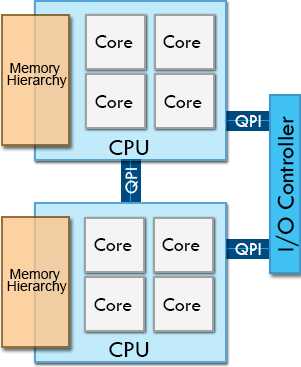
\includegraphics[scale=0.5]{../../common/img/numa_qpi.png}
		\caption{Schematic representation of a NUMA system with QPI interface.}
		\label{fig:CallgraphOriginal}
	\end{center}
\end{figure}

The \ttLoop is the main method of the application. Its purpose is to iterate through all events in the input file and perform 21 filtering and processing tasks (known as cuts) to each event. The most evident problem with the application, inherited from the LipMiniAnalysis library, is the non existence of a data structure on memory holding the events to process. Each input file has around 1 GByte that makes perfectly possible to be stored on RAM memory. However, for each event its information is read from the file and loaded to hundreds of global variables and then it is submited through the cuts. If all the events were read at once, it would be possible to take advantage of the higher bandwidth of sequential reads to the hard drive. Even the overhead of creating such data structure for the events would be compensated by the faster acesses and possibility of easier parallelization of the analysis at the event level, since the events have no dependencies between them.

Every method starting with a capital T refers to the ROOT framework. They are only being used for reading the input file and writing the results. The \ttDoCuts method performs the 21 cuts referred above. It is on cut 20 that \ttDilepKinFit is called, which becomes the most time consuming task as the number of variations per combination increases, as seen from table \ref{tab:TempoKinFit}, therefore, the efforts on improving the performance must be focused on this routine.

\begin{table}[!htp]
	\begin{center}
		\begin{tabular}{|c|c|c|c|c|c|c|c|c|c|c|c|}
			\hline
			\textbf{# of variations/combination} & 1 & 2 & 4 & 8 & 16 & 32 & 64 & 128 & 256 & 512 & 1024 \\ \hline
			\textbf{\% of time} & - & - & - & - & - & - & - & - & - & - & - \\ \hline
		\end{tabular}
		\caption{Percentage of the total execution time spent on the \ttDilepKinFit routine for various numbers of variations per combination.}
		\label{tab:TempoKinFit}
	\end{center}
\end{table}

\todo{terminar tabela com \% tempo na ttdilep}

\pdfbookmark{ttDilepKinFit Routine}{ttDilepKinFit routine}
\section{\ttDilepKinFit Routine}
\label{Application:ttDilepKinFit}

This routine has a main loop that calculates and iterates through all the possible combinations of jets and leptons for a given event. It is possible to define the number of variations to perform per combination, resulting in an inner loop. Some of the variables varied are local to the routine but most are global to the application. The kinematical reconstruction is performed inside the loops, for each variation of each combination and its results, as well as the bottom quarks not used, are used later in the Higgs boson reconstruction. A context is created when the combination to process is calculated, and its specific for the respective combination, which is altered by the variations, kinematical and the Higgs boson reconstructions. Each one of the solutions is stored in a vector and after all the combinations are computed, the said vector is iterated and only the best solution is choosen and its relevant data is copied to global variables.

The quality of a solution is dependent on two factors. The first is the accuracy of the kinematical reconstruction, which is measured by the probability of the reconstruction being properly performed, compared to theoretical models. The second is the accuracy of the Higgs boson reconstruction and its calculation is similar to the former. Since the Higgs boson reconstruction uses results of the kinematical reconstruction, namely the neutrinos and remaining bottom quarks, if the latter is faulty, i.e., performed with a low resultant accuracy, the Higgs boson will be poorly reconstructed too. The accuracy of the overall reconstruction of the event, for a given variance of a combination, is given by the probability of the kinematical reconstruction times probability of the Higgs boson reconstruction.

\begin{figure}[!htp]
	\begin{center}
		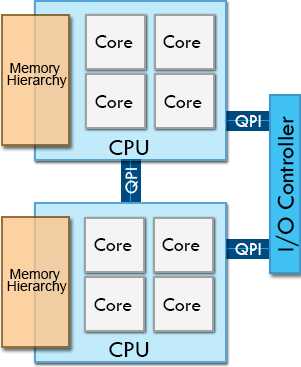
\includegraphics[scale=0.5]{../../common/img/numa_qpi.png}
		\caption{Callgraph of the \ttDilepKinFit routine.}
		\label{fig:CallgraphKinFit}
	\end{center}
\end{figure}

Note that the flow of \ttDilepKinFit may change between combinations, or even variations, within an event. The responsible of that behaviour is the \dilep routine. A certain combination may be capable of being reconstructed, both the \ttbar system and the Higgs boson, but with others the \ttbar system may not be reconstructable, which causes the \ttDilepKinFit flow to stop and process the next combination. This irregularity of the time that takes to process a combination can be problematic to the load balancing of the parallel tasks, as explained in section \ref{Parallelization:Sequential}.

The callgraph for the \ttDilepKinFit for 128 variations per combination is presented in figure \ref{fig:CallgraphKinFit}. The sections of the routine that are most relevant, the variation of the events parameters, the kinematical and Higgs boson reconstructions, are explained in depth in the next subsections.

\pdfbookmark{Variations Routine}{variations routine}
\subsection{Variations Routine}
\label{Application:Variations}

The purpose of the variation is to overcome the experimental resolution of the ATLAS detector, as explained in section \ref{Motivation}.The variation of the parameters of an event, for a given combination of jets and leptons, consists on applying an offset of a given magnitude to the said values. The offset is randomly obtained, using the TRandom3 pseudo-random number generator from ROOT, following a gaussian distribution. The mean value used is 0 and the standard deviation is 2\%, as it is the resolution error of the detector associated to every measurement. The values varied are the momentums of the 2 jets and 2 leptons that make the combination, and consequently their energy is recomputed.

The pseudo-random number generator used by the TRandom3 class is the Mersenne Twister \cite{MersenneTwister}, currently one of the most used generators for applications highly dependable on random numbers. This algorithm produces 32-bit uniformly distributed pseudo-random numbers with a period of $2^{19937}$. It has a relatively heavy state which is an integrant part on the algorithm flow. The generator is thread safe as long as different states are being used in different threads. The state can be shared among the threads but, however, change it must be done sequentially, sequentializing the number generation among the threads. In this case, the number generated by one thread will affect the number generated by the remaining.

\nvidia offers a parallel implementation of the Mersenne Twister for GPUs in the cuRand library \cite{NVIDIA:MersenneTwister}. It uses a precomputed set of 200 parameters, which can also be generated by the user, but offering a smaller period of $2^{11213}$. The pseudo-random number generation and state update is thread safe, up to 256 threads sharing the same state structure, for each block. Two different blocks can safely operate concurrently.

TRandom uses the Acceptance-Complement Ratio algorithm \cite{AcceptanceRandom} for transforming the pseudo-random numbers from an uniform to a gaussian transformation. It is allegely 66\% faster than the Box-Muller transformation \cite{BoxMuller} and similar to the Ziggurat method \cite{Ziggurat}. The cuRand library only offers the Box-Muller transformation with a basic pseudo-random number generator so, to accuratly replicate the results, it is needed to replicate the TRandom gaussian method on GPU using the cuRand implementation of Mersenne Twister.

\pdfbookmark{dilep Routine}{dilep routine}
\subsection{\dilep Routine}
\label{Application:dilep}

The kinematical reconstruction is performed in the \dilep routine. The \ttbar system obeys a set of properties of an theoretical expected model. To reconstruct both of the Top Quarks it is needed to know the characteristics of all resultant particles from their decay. However, since the neutrinos do not react with the detector, and their characteristics are not recorded, it is needed to infer them, using the properties of momentum and energy conservation of the system. Once the neutrinos characteristics are determined, it is possible to reconstruct the Top Quarks.

\dilep analitically solves a system of 6 equations to infer the neutrinos characteristics and then reconstruct the Top Quarks. The routine is dependent on only one class from ROOT, TLorentzVector, making it easy to port to GPU, aside from the process of marshaling and unmarshaling the data, namely the TLorentzVector classes from ROOT, into a format that is usable in \cuda. Executions of \dilep on different inputs are completely independent, since this function does not alter the global state of the \tth analysis.

\pdfbookmark{ttDilepKinFit Routine Computational Analysis}{ttDilepKinFit routine computational analysis}
\subsection{\ttDilepKinFit Routine Computational Analysis}
\label{Application:ttDilepKinFit:Analysis}

\todo{Coisas papi}
\pdfbookmark{Parallelization Approaches}{parallelization approaches}
\chapter{Parallelization Approaches}
\label{Parallelization:Sequential}

The section of code which takes more time is the \ttDilepKinFit function. The main objective is to run as many kinematical reconstructions per event, with a slight variation to the particle characteristics, and as they increase the \ttDilepKinFit execution time also increases. So, since it is the critical section of the application, the efforts on performance optimizations will be focused on this portion of the code.

The \ttDilepKinFit workflow can be divided in three main stages. Each event can have an arbitrary number of jets and leptons associated, requiring a minimum of two of each to perform the kinematical reconstruction of the \ttbar system. Events that not fulfill this requirement are discarded in the previous cuts. If there is more than the minimum number of jets and leptons it is necessary to combine them, in pairs of two jets with two leptons, and perform the kinematical reconstruction for every combination possible. Note that their order on the combination is not relevant, reducing the total amount of possible combinations. Then, it is possible to apply a variation to the jets and leptons characteristics, motivated by the reasons explained in section \ref{Motivation}. The variation has a magnitude equivalent to the experimental resolution of the ATLAS detector (which is 5\%) and it is applied to the three momentums and energy of the particles, and causing the need to re-compute other auxiliary parameters to the rest of \ttDilepKinFit. The number of variations to apply to each jet/lepton combination is arbitrary and defined by the user.

\ttDilepKinFit has a main loop, for each jet/lepton combination and for each variation of each combination, where the most intensive computation occurs, which will be explained next, and a final section of code that iterates through all the reconstructions and picks only the best, discarding all the others computed.

Inside the main loop of \ttDilepKinFit is possible to identify three distinct stages of the reconstruction. The first is the variation of the jets and leptons momentums, as explained before. The second stage is the kinematical reconstruction of the \ttbar system, using the varied combinations. It attempts to reconstruct the \ttbar system, presented in section \ref{Motivation} and produces a result (the Top Quarks), which has an computed probability associated to its accuracy. This probability determines the quality of the reconstruction. The third stage is the reconstruction of the Higgs boson, using the results of the kinematical reconstruction. This reconstruction also has a probability associated, and the final quality of the overall reconstruction of the event is given by the multiplication of this probability with the one of the kinematical reconstruction of the \ttbar system. Figure \ref{fig:SeqPipeline} presents the explained workflow of \ttDilepKinFit.

\begin{figure}[!htp]
	\begin{center}
		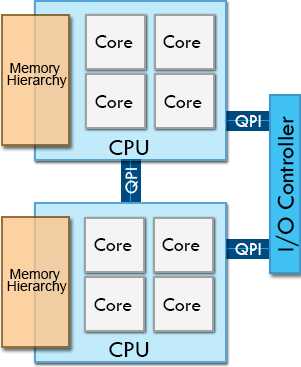
\includegraphics[scale=0.5]{../../common/img/numa_qpi.png}
		\caption{Schematic representation of the \ttDilepKinFit workflow.}
		\label{fig:SeqPipeline}
	\end{center}
\end{figure}

Note that there is data dependencies between loop iterations, since that for chosing the next jet/lepton combination it is necessary to know which combinations were already picked, and between the three stages within the loop. The kinematical reconstruction needs the combination already varied, and the Higgs boson reconstruction needs the result from the kinematical reconstruction in order to chose different particles (since one particle cannot belong to the \ttbar system and the Higgs boson decay). The current workflow is not suitable for parallelization.

A generalist workflow suited for parallelization is presented in figure \ref{fig:ParallelPipeline}. The combinations must be computed, and also all the variations, and their information stored in a data structure, so that the main loop of \ttDilepKinFit is eliminated. Now, each stage of the workflow can have its own loop, which is not represented in the figure since it is considered to be part of the stage itself. By having their own loop, the stages can now be executed in parallel, but maintaining the same data dependencies between stages.

\begin{figure}[!htp]
	\begin{center}
		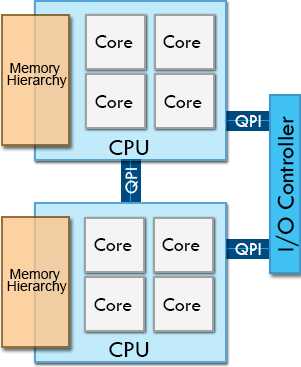
\includegraphics[scale=0.5]{../../common/img/numa_qpi.png}
		\caption{Schematic representation of the \ttDilepKinFit workflow.}
		\label{fig:ParallelPipeline}
	\end{center}
\end{figure}

\pdfbookmark{Shared Memory Parallelization}{shared memory parallelization}
\section{Shared Memory Parallelization}
\label{Parallelization:SharedMem}

The parallel workflow model proposed for this implementation is similar to the generalist previously presented. One challenge to the implementation is that most of the variables are global to the application, and there is no data structure holding the information needed during \ttDilepKinFit, such as the combinations. The computation of the jet/lepton combinations must be kept sequential, since choosing one combination is always dependent on all the previous combinations made and, therefore, cannot be parallelized. The final iteration through all the results, in which the best solution is chose and is ``uploaded'' to global variables, cannot also be parallelized in the current implementation (there is, however, a way to overcome part of this problem that will be explained later). During this chapter a concurrent task is considered to be the subset of a parallel region. The aggregation of all these tasks is the whole parallel region. Figure \ref{fig:SharedMemPipeline} presents the workflow used for this implementation, and is explained next.

\begin{figure}[!htp]
	\begin{center}
		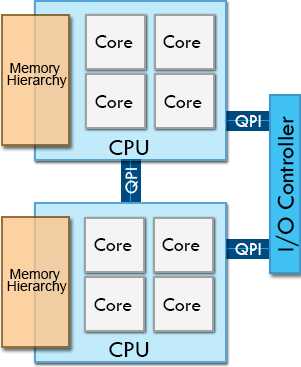
\includegraphics[scale=0.5]{../../common/img/numa_qpi.png}
		\caption{Schematic representation of the \ttDilepKinFit workflow.}
		\label{fig:SharedMemPipeline}
	\end{center}
\end{figure}

In this implementation it does not make any sense to use different tasks for different stages that can be parallel; two of the three steps presented next that can be parallel will be aggregated in the same task, increasing its granularity and reducing the number of synchronizations necessary between tasks. The first step of the new workflow is to create a data structure holding all the combinations and other information associated with them. Each task will pick the respective combination and perform a loop over the subset of the total number of variations. The grain size of the parallel work of each task will be dependent on the total number of combinations times the number of variations per combination (the higher this value the coarser the grains size) and the number of parallel tasks (the higher the number of tasks the thinner the grain size).

The second step, the kinematical reconstruction of the \ttbar system, will be performed within the same task, meaning that there is no synchronization between this and the previous steps among different tasks. The same happens between this and the third step, the Higgs boson reconstruction. By aggregating these three steps the grain size of the tasks is increased, compared to the generalist parallelization model presented before, which benefits their execution on CPU (a lesser number of coarser tasks means that the CPU spends more time performing computations relevant to the application and less time switching context, which is very slow).

As explained before, after these three stages, on the original workflow, there is an iteration through all the solutions and the best is chosen. Instead of saving all the solutions, after each iteration of the loop of the current workflow the solution is compared to the previous and only the best of the two is save. When all tasks finish all their respective iterations, each will have the best solution for the subset of combinations and variations that they processed. A reduction can be made so that the best solution from all the tasks is found. However, another data structure must be created, since the best solution is a set of variables and TLorentzVectorWFlags (from the LipMiniAnalysis library) class instances. The final ``uploading'' of the best solution to global variables is only made by the task with the best solution.

This workflow will have two limitations to the performance scalling, the creation of the data structure holding the combinations and the best solutions and the creation and work sharing between the tasks. Its time increases with the number of combinations and variations and the number of parallel tasks to use.
%\pdfbookmark{Implementation and Performance Analysis}{implementation and performance analysis}
\chapter{Implementation and Performance Analysis}
\label{Implementation}

In this chapter the implementation process, based on the models on section \ref{Parallelization:Sequential} of the different approaches will be presented and discussed. After explaining all the details of the implementation for a given platform an analysis from the computational point of view will be presented, along side with the performance comparison of the said implementations. Finally, a comparative analysis of all the implementation will be presented.

\pdfbookmark{Shared Memory Implementation}{shared memory implementation}
\section{Shared Memory Implementation}
\label{Implementation:SharedMem}

The implementation of the shared memory parallelization follows the workflow presented in section \ref{Parallelization:SharedMem}. The first goal was to have a working na\"{i}ve implementation that could be used as a starting point so that it could be profiled and the bottlenecks identified.

The first step was to divide the \ttDilepKinFit main loop that iterates through all the combinations of leptons/jets of an event, and then the respective variations, exemplified in the workflow of section \ref{Parallelization:Sequential}. The first problem with this approach is that the portion of the code to parallelize reads and writes in a set of 34 global variables, most of them being vectors of ROOT classes. The access to these variables could be controlled in such a way that only one thread would be writing on the said variables. However, they would have to do it in order to ensure that the state of the reconstruction of one variation would not mix with others. A much simpler way is to create a copy of the said variables for each thread to work on. This avoids serial access to the variables which would cause contention and degrade the performance.

The second problem is that the various combinations, and respective variations, must be scattered among the threads so that each has a data set to work on. Each combination, and respective variations, are also stored in global variables, but these cannot be simply made private to each thread. The portion of \ttDilepKinFit that build the combinations cannot be parallelized because the computation of a given combination is dependent on the jets and leptons used in the previous to avoid duplicates. The total amount of combinations, which depends on the amount of jets and leptons, $n$, (regardless of the order, i.e., $(j_1, j_2) = (j_2, j_1)$), pairing two jets with two leptons in the same combination, with $k = 4$, is, according to the mathematical formula for combinations \ref{eq:Combination}:

\begin{center}
	\begin{equation}
		\binom{n}{k} = \frac{n!}{k!(n - k)!} \mbox{, with k = 4 then } \binom{n}{4} = \frac{n!}{8(n - 4)!}
		\label{eq:Combination}
	\end{equation}
\end{center}

On average, the number of combinations for each event that reachs the cut 20 with the given input is \todo{QUANTO E?}.

For the combinations to be scattered among the threads it is needed to store them in a data structure, instead of using global variables as it is currently implemented, and then each thread picks a combination and processes it. The implementation and other specific details of the data structure is presented in subsection \ref{Implementation:SharedMem:DataStructs}.

Furthermore, only the best reconstruction is used so there is no need to store all the reconstructions

\todo{seccao para a estrutura de dados e calcular o seu tamanho etc)

\pdfbookmark{Data Structure Characterization}{data structure characterization}
\subsection{Data Structure Characterization}
\label{Implementation:SharedMem:DataStructs}
\chapter{Conclusions \& Future Work}
\label{ConclusionFutureWork}

\begin{quote}
\textit{This chapter concludes the dissertation, presenting an overview of the results obtained by the work developed, on both homogeneous and heterogeneous systems. Guidelines for future work, on improving the test case application and providing parallel solutions abstracted from the programmer for future application development, are presented.}
\end{quote}

\section{Conclusions}
\label{Conclusion}

This dissertation presents 4 different approaches to increase the performance of a scientific application that processes event data gathered at ATLAS, developed by the LIP physics research group, using homogeneous and heterogeneous systems, testing in the latter 2 different hardware accelerators. The objective is to evaluate the usability, performance and efficiency of the different systems and specific accelerators, as well as the quality and structure of the application and libraries.

The scientific application attempts to reconstruct the Top Quarks and Higgs boson that decay from a head-on collision of two protons, based on the resultant data collected in the ATLAS particle detector at the LHC. The quality of the reconstruction depends on the amount of partial reconstructions performed, with the event parameters slightly varied, with the purpose of overcoming the experimental resolution of the particle detector and find the most accurate final reconstruction. However, increasing the number of partial reconstructions directly affects the application execution time, decreasing the number of events processed and impacting the researched conducted by LIP.

An initial optimization of the pseudo-random number generator, in which the application relies heavely, is proposed. Then, 4 parallel implementation solutions were developed, based on an identification of the critical region restricting the performance. Two implementations target heterogeneous systems with accelerator devices, one using an \nvidia GPU and other using the \intel Xeon Phi. Both implementations face many limitations, primarly due to the abscence of a data structure holding all the event information on both the application and LipMiniAnalysis, restricting the performance gains and efficient usage of the GPU. Also, due to this hardware limitations, only part of the application critical region was parallelized on the accelerator, increasing the amount of high latency memory transfers between CPU and GPU, and forcing the rest to be parallelized on CPU.

The parallelization on the \intel Xeon Phi had the purpose of evaluating its performance, but more importantly, its usability, as \intel advertises easy porting of CPU code to the device. The objective was to test the Xeon Phi in both native and offload modes. One of the application dependencies, ROOT library developed by CERN, is supposed to have support for this device but, it did not work and many hours were spent trying to solve the problem. Using the device in offload mode, similar to the GPU, would require that only part of the critical region is parallelized, as it depends on many functionalities of ROOT that cannot be simultaneously compiled for CPU and Xeon Phi. Its resources would also be inefficiently used due to the lack of a global data structure with all events. Even though the parallelization implementation is simplified by the use of pragma directives available for this device, the driver offered many limitations due to the computational complexity of the portion of the code to parallelize. The Xeon Phi is still new to the market, causing its drivers and libraries to not be completely stable. Many of the errors provided by the drivers were not even documented yet. Due to the dissertation timeframe, both implementations were left on hold, with the only conclusion that the device is not mature enough to provide an easy porting of the code for real applications, opposed to \intel claims.

The remaining 2 parallel implementations were aimed towards homogeneous systems, which constitute all of the LIP computational resources. The first was a shared memory implementation, from which two versions derived. One has a smaller parallelization overhead and better performance on single-socket systems, while the second, with a bigger overhead, but performing better on multi-socket systems. The second implementation is a application scheduler, oriented for multi-socket systems. The idea was based on the efficient use of computational resources of the first version of the shared memory implementation on a single CPU. Multiple instances of this application, processing different input data files, would provide an efficient use of all available computational resources and an even bigger increase in performance, compared to the shared memory implementations. A prototype was developed and tested with promissing results, but its performance is still manually tuned by a set of parameters which may vary from system to system. The scheduler is prepared to work with any kind of scientific application, only requiring that multithreaded applications use a given API to be configured.

The lack of structure on the code of both the application and LipMiniAnalysis library restricted the performance on heterogeneous systems. The best performance was attained for a shared memory implementation on homogeneous systems and, allied to the use of a prototype scheduler, provided an efficient use of the available resources. The LIP research group has the best interest in these implementations as they increase their productivity and do not require investment in expensive hardware accelerators.

\section{Future Work}
\label{FutureWork}

The results obtained in this dissertation, specially for the implementations on heterogeneous systems and the application scheduler, motivates further work on this theme. The application scheduler is on the best interest of the LIP research group and, if its development continues, it may be widely used among the researchers. Guidelines for continuing this dissertation work may include:

\begin{itemize}
	\item Restructuration of the LipMiniAnalysis library, creating a data structure holding all the event information in the input data file. These files are usually 1 GB size, which is perfectly capable of being stored in RAM memory. It would allow a more efficient implementation of this kind of applications on heterogeneous systems with hardware accelerators.
	\item Refining the GPU implementation using the new restructured version of LipMiniAnalysis and analyze if the potential performance gains justify investment from the LIP group on this hardware and academic formation on programming for these devices.
	\item Explore parallelism on heterogeneous systems using parallelization frameworks, such as OpenACC.
	\item Refining the application scheduler prototype by:
	\begin{itemize}
		\item Implementing and validating the remaining features for working with any kind of scientific application;
		\item Validating its capability of scheduling different applications on the same system;
		\item Overall load balancing optimizations by refining current mechanisms, such as implementing specific core binding of the applications;
		\item Implementing micro-benchmarks to evaluate the computational system and generate the best setup, considering the computational characteristics of these applications.
	\end{itemize}
	\item Parallelization of the restructured LipMiniAnalysis. Since the library serves as a skeleton for many of the LIP applications, a parallelization at the event level would allow high performance and efficient applications to be developed by physicists without requiring the programming know-how to extract parallelism on homogeneous platforms.
\end{itemize}

%\appendix
\chapter{Test Environment}
\label{App:TestEnv}

This appendix focuses on characterizing the hardware and software used in all performance measurements of the application for the different implementations developed.

Four dual-socket multicore systems with CPUs of different architectures on the SeARCH cluster were used to test the shared memory implementation, with the purpose of testing a wide range of systems commonly available in small physics research group clusters. The first, named compute-711 node, has two \intel Xeon E5-2670 (Sandy Bridge architecture) \cite{Intel:E52650}, using the Quick Path Interconnect (QPI) interface between CPUs, in a Non Unified Memory Access model (NUMA), meaning that the latency of a CPU acessing its own memory bank is lower than accessing the other CPU memory bank. The QPI interface can perform up to 8 GT/s (giga transfers per second) of 2 bytes packets, in each of the two unidirectional links, for a total bandwidth of 32 GB/s. The system features 64 GB of DDR3 RAM with a speed of 1333 MHz, for a maximum bandwidth of 52.7 GB/s. All RAM bandwidths were measured using the STREAM benchmark \cite{STREAM}.

The second system, named compute-601 node, has the same amount of RAM at the same speed, with a maximum bandwidth of 28.6 GB/s. The two CPUs are \intel Xeon X5650 (Nehalem architecture). The difference of memory bandwidth is due to the different memory controllers, with the one in Nehalem having 3 memory channels, as opposed to the 4 memory channels in the Sandy Bridge CPUs. The two CPUs are interconnect by a QPI interface, but with a different speed than the Sandy Bridge, performing 6 GT/s in each of the two unidirectional channels, for a total bandwidth of 24 GB/s.

The third system is also powered by an \intel processor, the compute-401 node, with 8 GB RAM and a maximum bandwidth of 18.4 GB/s. The CPUs are the Xeon E5520 (Nehalem architecture). The two CPUs are interconnected by a QPI interface with the same bandwidth of 24 GB/s.

The fourth system features two \amd Opteron 6174 CPUs, being the system with the most physical cores. It has 64 GB of DDR3 RAM at 1333 MHz, with a maximum measured bandwidth of 39.8 GB/s. \amd uses HyperTransport (HT) 3.0 technology, a point-to-point interconnection similar to QPI capable of transmitting 4 byte packets through two links, for an aggregate bandwidth of 51.2 GB/s. The characteristics of the CPUs on the three systems are presented in table \ref{tab:CPUS}.

\begin{footnotesize}
\begin{table}[!htp]
	\begin{center}
	\smaller
		\begin{tabular}{|c|c|c|c|c|}
			\hline
			\textbf{System} & compute-711 & compute-601 & compute-401 & compute-511 \\ \hline
			\textbf{CPU} & \intel Xeon E5-2670 & \intel Xeon X5650 & \intel Xeon E5520 & \amd Opteron 6174 \\ \hline
			\textbf{Architecture} & Sandy Bridge & Nehalem & Nehalem & Magny\-Cours \\ \hline
			\textbf{Clock Freq.} & 2.60 GHz & 2.66 GHz & 2.3 GHz & 2.2 GHz \\ \hline
			\textbf{\# of Cores} & 8 & 6 & 4 & 12 \\ \hline
			\textbf{\# of Threads} & 16 & 12 & 8 & 12 \\ \hline
			\textbf{L1 Cache} & \specialcell{32 KB I. +\\32 KB D. per Core} & \specialcell{32 KB I. +\\32 KB D. per Core} & \specialcell{32 KB I. +\\32 KB D. per Core} & \specialcell{64 KB I. +\\64 KB D. per Core} \\ \hline
			\textbf{L2 Cache} & 256 KB per Core & 256 KB per Core & 256 KB per Core & 512 KB per Core \\ \hline
			\textbf{L3 Cache} & 20 MB shared & 12 MB shared & 8 MB shared & \- \\ \hline
			\textbf{CPU Interconnection} & QPI @4.0 GHz & QPI @3.2 GHz & QPI @3.2 GHz & HT @3.2 GHz \\ \hline
			\textbf{ISE} & AVX & SSE 4.2 & SSE 4.2 & SSE 4a \\
			\hline
		\end{tabular}
		\caption{Characterization of the CPUs featured in the three test systems.}
		\label{tab:CPUS}
	\end{center}
\end{table}
\end{footnotesize}

The \nvidia Tesla C2070 has 14 Streaming Multiprocessors (SM) with 32 CUDA cores each, making a total of 448 CUDA cores running at a clock frequency of 1.15 GHz. Each SM has 64 KB of L1 cache, with two configurations for private cache and shared memory for the CUDA threads inside a block (16 KB / 48 KB and vice-versa). The 768 KB of the L2 cache is shared among all SMs. The GPU board features 6 GB of GDDR5 memory. \nvidia claims a theoretical peak performance of 1.17 TFLOPS (double precision floating point arithmetic).

The \intel Xeon Phi has 60 multithread cores, with 4 threads per core, running at a clock frequency of 1 GHz. It has an aggregated L2 cache size of 30 MB, spread among all cores. The private L1 cache has 64 KB size for data and another 64 KB for instructions. The cores communicate using a bidireccional ring network. The chip has 8 GB GDDR5 memory, capable of a bandwidth of 320 GB/s.

The GNU compiler version 4.8 was used with the -O3 optimizations and the AVX/SSE 4.2/SSE 4a instruction set (depending on the CPU architecture) where the compiler sees fit. The \intel Compiler (ICC) version 13.1 was used for the \intel Xeon Phi implementation. Both compilers feature the OpenMP version 3.2 used in the shared memory implementation. The GPU implementation required the use of the CUDA 5 SDK, in conjunction with the GNU compiler version 4.6.3 for the code to run on the CPU (any later versions are not supported by the \nvidia NVCC compiler). The ROOT \cite{CERN:ROOT} version 5.34/05 was used. The Performance API version 5.0 was used to measure the hardware counters of the CPU to the characterize the \ttDilepKinFit function.

\appendix
\pdfbookmark{Theoretical Performance Models}{theoretical performance models}
\chapter{Theoretical Performance Models}

\section{Amdahl's Law}
\label{AmdahlsLaw}

The speedup that can be achieve by parallelizing an application is not only dependent on the number of parallel tasks but also on the percentage of the code that will run in parallel. This means that it is possible to have an extremely optimized implementation of the parallelization but if only a small part of the code is parallel the speedup will be small.

Amdahl's Law \cite{AMDAHL} defines the maximum attainable speedup of parallelizing an application, comparing a multithreaded application using $N$ processors with its serial counterpart. The law takes into account the portion of the code, $P$, that can be paralelized and defines the maximum speedup $S$ that can be obtained.

\begin{center}
	\begin{equation}
		S(N) = \frac{1}{(1 - P) + \frac{P}{N}}
		\label{eq:Amdahl}
	\end{equation}
\end{center}

Equation \ref{eq:Amdahl} defines the maximum attainable speedup resultant from the parallelization of an application according to the Amdahl's Law. The law is used in this work to prove that the small speedups for fewer number of variations per event are close to the theoretical maximum and are limited by the percentage of the code that can be made parallel.

\section{Roofline Model}
\label{App:Roofline}

The Roofline model \cite{Roofline} was used characterize the system in terms of attainable peak performance. This model uses two metrics for the performance calculation: the peak CPU performance and the memory bandwidth. With the peak values of these two metrics a roofline is drawn, being the theoretical limit for the performance on the system. Then, other ceilings can be added, which further limit the maximum attainable performance. The classic Roofline uses float point computation as the peak CPU performance metric, which is usually advertised as peak performance by CPU manufacturers. It may be a good metric for heavy computational algorithms, such as matrix multiplication, but the type operations on the critical region (\ttDilepKinFit function) are much more varied, as shown by the instruction mix presented in section \ref{ComputationalCharactrization}. Instead, the computational intensity was used for measuring the CPU peak performance, as it considers all types of instructions.

The peak computational intensity is calculated with the formula \ref{eq:CompIntensity}. The clock frequency and number of cores are easily obtained by consulting the CPU specifications, while the number of instructions issued per clock cycle is more difficult to obtain. It is based on the super scalarity degree of the processor, i.e., the number of instructions that can be decoded per clock cycle, and then it must be confirmed if it matches with the number of arithmetic/memory units.

\begin{center}
	\begin{equation}
		C = Clock Freq. * # of Cores * # of Instructions per Clock
		\label{eq:CompIntensity}
	\end{equation}
\end{center}

The tilted ceiling of the Roofline model refers to the maximum memory bandwidth of the system and it was determined using the stream benchmark. The values are presented in appendix \ref{App:TestEnv}.

Figure \ref{fig:Roofline} illustrates the Roofline model for the four systems used.

\todo{Rooflines...}

%\appendix
\chapter{Test Methodology}
\label{App:TestMethodology}

The purpose of this appendix is to present the methodology used to conduct all tests related to the performance and algortihm characterization.

All tests use the same application input data file containing 5738 events, from which 1867 reach the \ttDilepKinFit and the rest are discarded in the previous cuts, of a proton-proton collision. The problem size is considered to be the number of variations to do to each combination of the jets and leptons within an event. The number of variations tested was $2^{x}$, where $x \in \{1, ..., 9\}$.

Various number of threads were used to conduct the tests of the shared memory implementations, depending on the system to run. The test using 1 thread has the purpose of evaluating the overhead of the creation and access to the data structures, as well as other implementation details relative to the parallelization. There is always one test using more threads than available by the hardware and its purpose is to test if the software multithreading (managed by the operating system) has benefits, which can expose memory access problems. The number of threads equal to the number of cores in one CPU tests the application without the limitations of the NUMA memory accesses and multithreading. With the number of threads equal to the total number of cores tests the use of both CPUs without hardware multithreading. The number of threads equal to the available hardware threads tests both CPUs with hardware multithreading active.

The number of used threads in the GPU is equal to the number of variations times the number of combinations, so that each thread computes a variation of a combination. This provides a high number of threads to hide the latency of memory accesses of the GPU.

%The tests on the \intel Xeon Phi were conducted on its two different operating modes: native and offloading. In the native mode all the application is executed on the device, as it is possible to use the ROOT and LipCbrAnalysis libraries since the device uses x86 code, even the single threaded portion of the code. Only the accesses to read the data from the hard drive pass by the CPU. In the offloading mode the Xeon Phi acts like a regular GPU, where only a portion of the application code is executed on the device.

It is important to adopt a good heuristic for chosing the best measurement since it is not possible to control the operating system and other background tasks, which can occasionally interfere with the measurements. The mean value is very sensitive to extreme measurements, i.e., the cases when the system has a spike on the workload from other OS tasks and it impacts the measurement, not accurately reflecting the actual performance of the application. The median can be affected by a series of values measured while the system in under load. Chosing only the best measurement, is not a solid heuristic, since it is more hard to replicate the result.

The chosen heuristic was the \textit{k best} methodology. It accepts the best value within a given range of other \textit{k} measurements. It is almost as good as the best value heuristic for obtaining the best measurement, but offers a solid result capable of being replicated. Was used a 5\% interval with a \textit{k} of 4, for a minimum of 16 measurements and a maximum of 32 (in case that there are less than \textit{k} values within the interval).

The \texttt{gettimeofday} function from the C standard libraries was used to measure the execution time of the application and its functions, providing microssecond precision. It is precise enough considering that the original application always takes more than 3 seconds to execute on all the used test systems. CUDA Events were used for measuring the portion of the code executed on the GPU, ensuring that the times were properly recorded and by synchronizing the kernel execution.



%\bibliographystyle{../../common/IEEE}
%\nocite{*}
\newpage % force the bookmark to go to the new page
\pdfbookmark{References}{references}
\printbibliography[title=References]

\end{document}
